%This file contains the LaTeX code of my laboratory report for my Database course.
%Author: 周芯怡/Xinyi Zhou <17307130354@fudan.edu.cn>
%Author: 张作柏/Zuobai Zhang <17300240035@fudan.edu.cn>

\section{项目特点}

Mini-CS Ranking的主要设计目的是创建一个便捷的学术检索平台,并提供友好的用户交互界面。其主要特征有:

\begin{itemize}
\item {\bf 学校排名功能}:Mini-CS Ranking模仿了CS Rankings的主要功能,即根据发表论文数量对学校进行排名。

\begin{figure}[h]
\centering
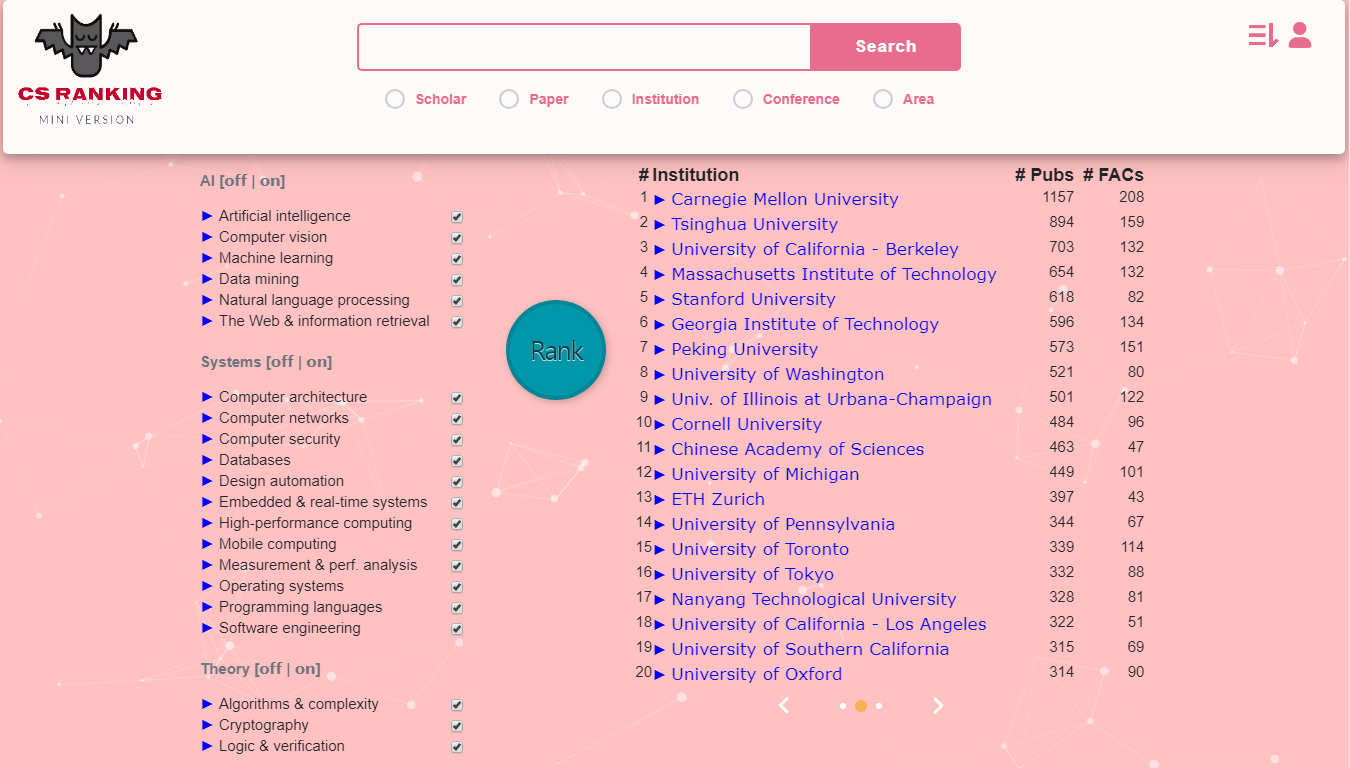
\includegraphics[width=0.8\textwidth]{asset/ranklist.png}
\end{figure}

$\quad$在排行榜中,可以看到学校的排名、发表论文数量和教师数量。点击左侧蓝色三角,即可看到学校下的老师排名。所有排名均是根据老师、学校发表的论文数量来降序排序的。老师的信息中还显示了老师所在的领域、老师的首页、老师的GoogleScholar页面和DBLP页面。

$\quad$左侧是领域的信息,点击领域旁的蓝色三角,可看到属于该领域的顶会。勾选所关心的领域,点击Rank按钮,即可在排行榜中筛选出相关领域的老师。

\item {\bf 信息检索功能}:

\begin{figure}[h]
\centering 
\subfigure{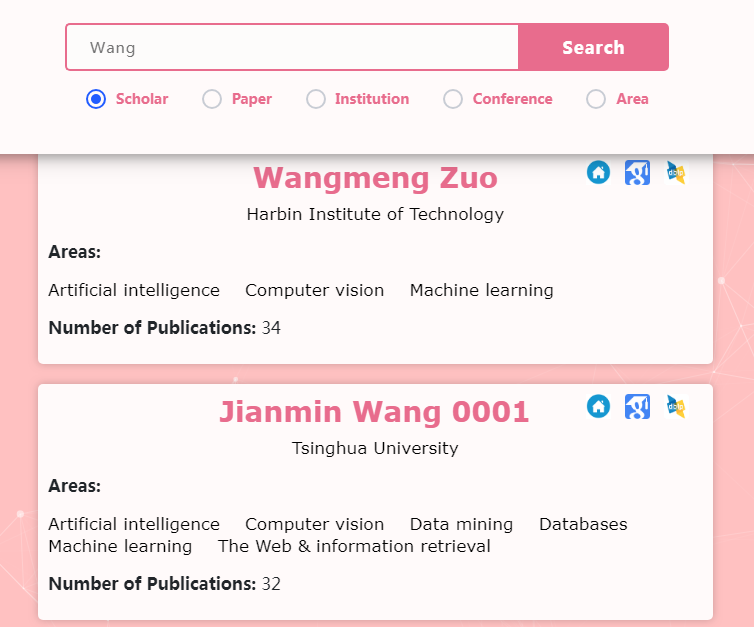
\includegraphics[width=0.4\textwidth]{asset/search_scholar.png}}
\hspace{1cm}
\subfigure{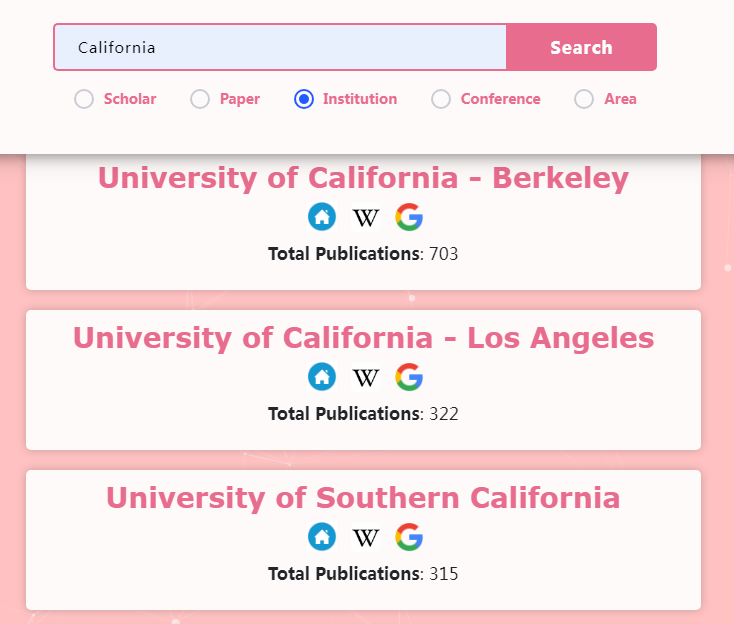
\includegraphics[width=0.4\textwidth]{asset/search_institution.png}}
\end{figure}

$\quad$为了便于检索自己感兴趣的老师,我们设计了类似GoogleScholar的搜索功能。可以通过勾选搜索框下的选项,并输入搜索关键词来检索学校、论文、老师。并且,我们为每个学校和学者都设计了自己的主页。学者的主页中包含其近几年发表的论文、每年发表的论文数量和他的合作者。学校的主页中,则详细的列举了该校的学者信息,并统计了近几年中各个领域发表论文的数量。

\item {\bf 领域会议信息}:除了上面提到的几项,我们还模仿DBLP,提供了会议和领域的检索功能,为相关领域的学者提供便利。


\begin{figure}[h]
\centering
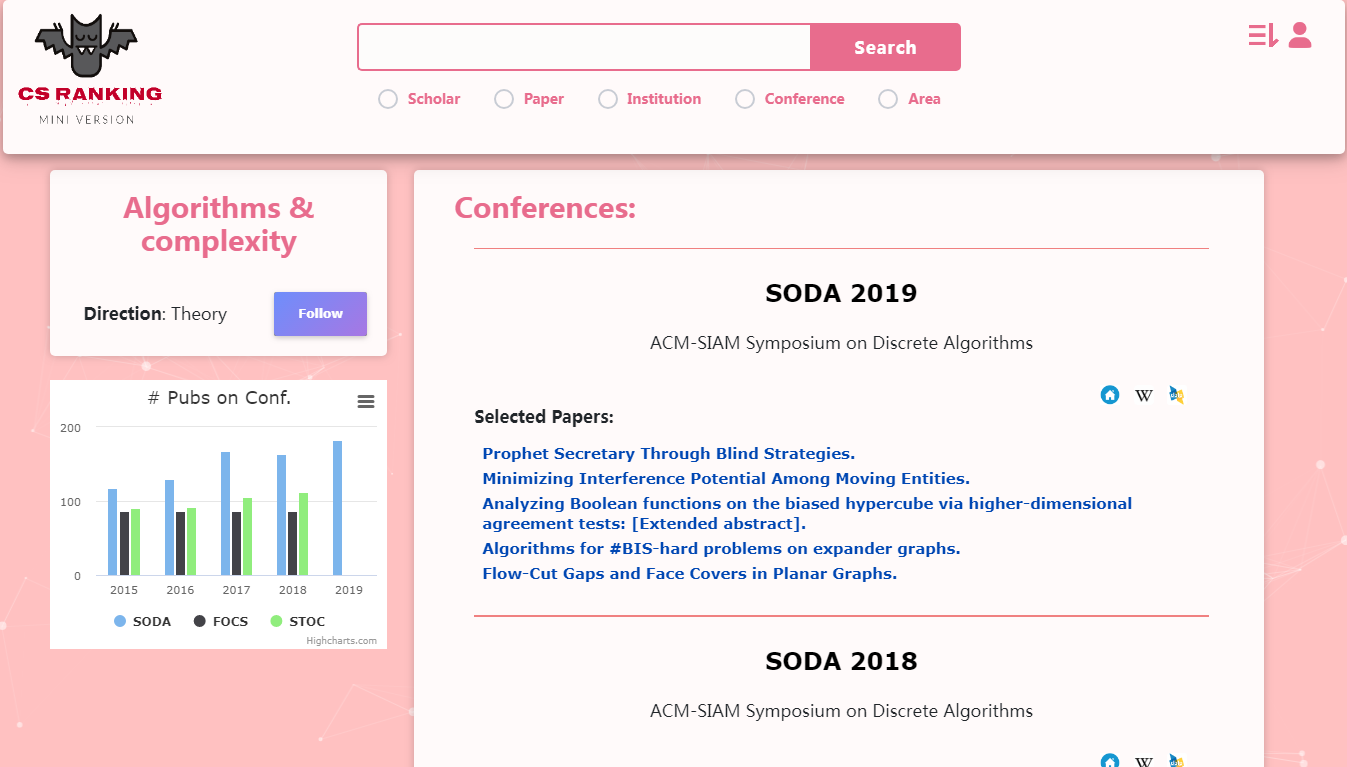
\includegraphics[width=0.75\textwidth]{asset/area.png}
\end{figure}

$\quad$在会议的相关主页中,我们给出了该会议的所有论文,并提供了访问会议首页与DBLP的链接。在领域的主页中,我们则列举了该领域的顶级会议,统计了近几年来会议中的论文数量,并给出了几位近五年来领域最活跃的学者。

\item {\bf 用户关注功能}:为了提升用户友好性,我们设计了关注功能,用户可以在相应主页关注自己感兴趣的学者、院校、领域等。这样一来,访问各主页就无需每次重新进行搜索,更加便捷;同时,当关注的学者发表新的论文时,会收到系统发来的消息提醒。

\begin{figure}[h]
\centering
\subfigure{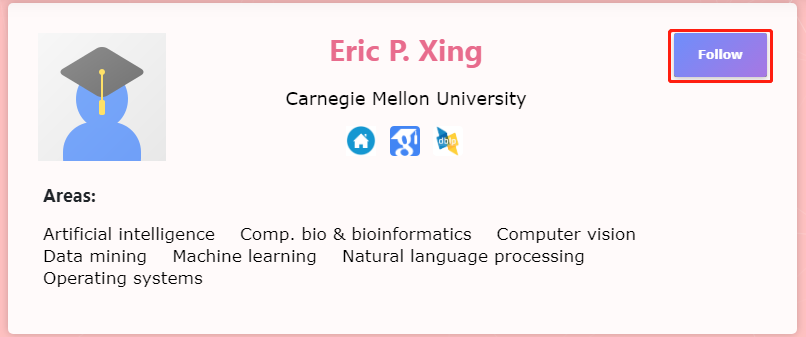
\includegraphics[width=0.6\textwidth]{asset/follow.png}}
\hspace{0.3cm}
\subfigure{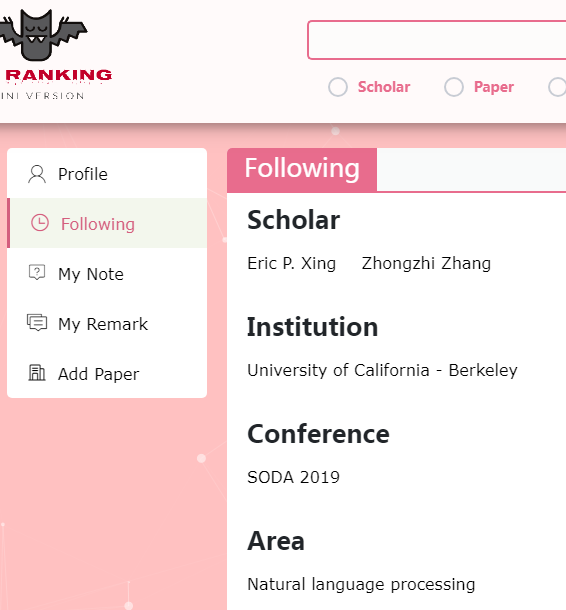
\includegraphics[width=0.35\textwidth]{asset/following.png}}
\end{figure}

\item {\bf 认证发表论文}:用户注册时,若系统检测到数据库中有姓名相似的学者,则会进行学者认证。认证后,学者的信息会自动导入用户信息中,并获得发表新论文的权限,成功发表论文后,则会通知该学者的所有关注者。

\begin{figure}[h]
\centering
\subfigure{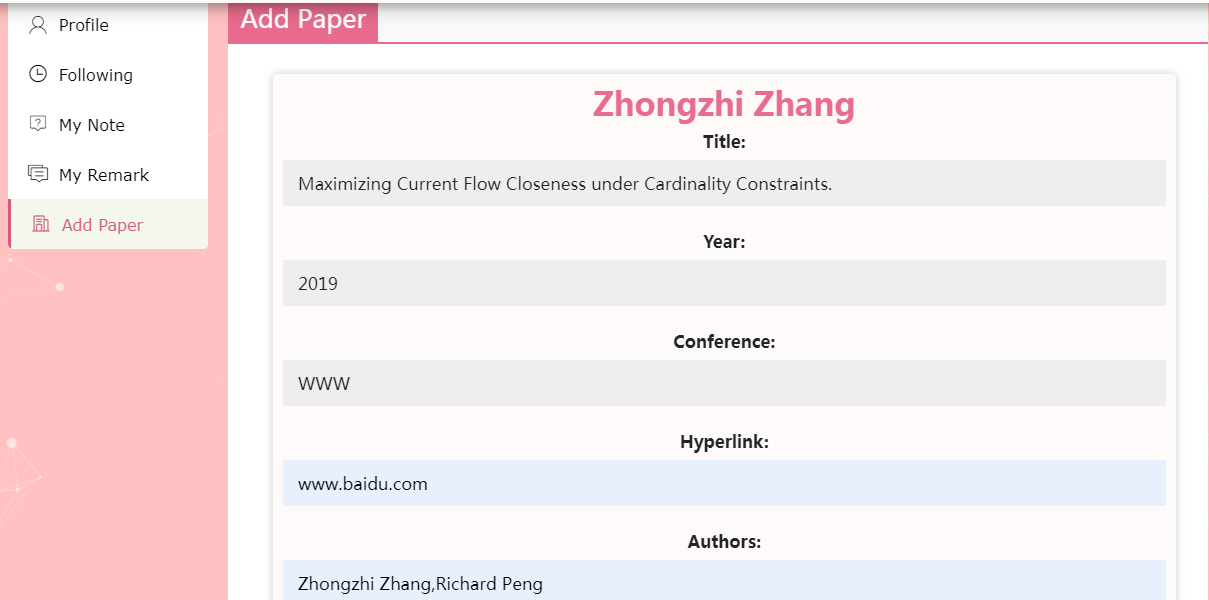
\includegraphics[width=0.6\textwidth]{asset/add_paper.png}}
\hspace{0.3cm}
\subfigure{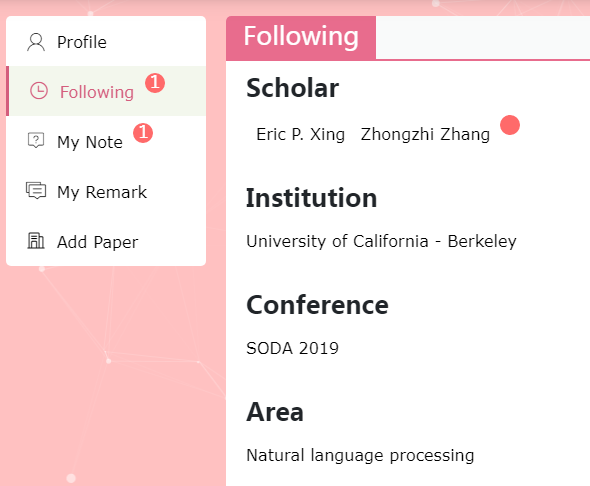
\includegraphics[width=0.35\textwidth]{asset/new_following.png}}
\end{figure}

\item {\bf 书写笔记评论}:登录后,用户可以就自己感兴趣的论文书写笔记,并会显示在论文主页下方。进入笔记主页可发表评论,笔记作者则会接收到新评论的提醒信息。

\begin{figure}[h]
\centering
\subfigure{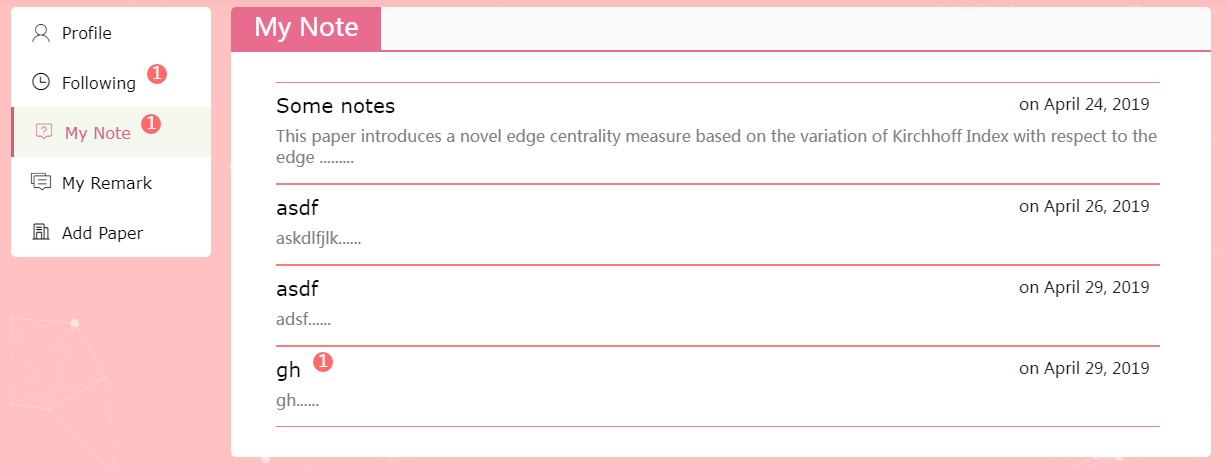
\includegraphics[width=0.9\textwidth]{asset/new_note.png}}
\end{figure}

\end{itemize}

因此,可以说,Mini-CS Ranking集合了CSRankings,GoogleScholar,DBLP三者的核心功能,又增加了友好的用户登录功能,并提供了更为美观的交互界面。


